\documentclass[12pt]{article}

% Load packages
\usepackage[top=1in, bottom=1in, left=1in, right=1in]{geometry}
\usepackage{graphics}
\usepackage{graphicx}
\usepackage{epsfig}
\usepackage{epsf}
\usepackage{epstopdf}
\usepackage{mathrsfs}
\usepackage{amsmath}
\usepackage{amssymb}
\usepackage{textcomp}
\usepackage[scaled=.90]{helvet} % Helvetica (currently not used)
\usepackage[]{lineno} % For line numbers

% Define new commands and definitions
\def\ds{\displaystyle}
\def\d{\partial}
\newcommand{\rr}{\mathbb{R}}
\newcommand{\zz}{\mathbb{Z}}
\newcommand{\nn}{\mathbb{N}}
\newcommand{\ee}{\mathscr{E}}
\newcommand{\mb}{\mathbf}
\newcommand{\ol}{\overline}

% Text formatting
\linespread 2	
\linenumbers

\title{Escape direction does not matter for some fish prey}
\author{Matthew J. McHenry, Alberto Soto}
%\date{}                                           % Activate to display a given date or no date

\begin{document}
\DeclareGraphicsExtensions{.eps,.pdf,.png,.gif,.jpg,.ps}

\maketitle

\pagebreak


% ABSTRACT
% --------------------------------------------------------------------------------
\begin{abstract}

Abstract text...

\end{abstract}

\pagebreak


% --------------------------------------------------------------------------------
\section{Introduction}

Biologists have long-appreciated the importance of predation in the ecology and evolution of prey. The subject is extensive enough to fill the pages of books on the fascinating diversity of strategies prey use to avoid encounters with predators (CITE) or the defenses employed (CITE) when discovered. However, much less attention has focused on understanding how a tremendous diversity of prey evade capture by locomotion. In this area, the direction of motion is considered to be critical in over the short timescale of an encounter with a predator (CITE). The present paper examines the strategic implications of directed motion by comparing the predictions of a game theory model (CITE) with experimental results on predator escape in larval zebrafish (\textit{Danio rerio}) (CITE).

Studies on locomotion commonly speculate on the implications of locomotor performance for predator evasion. Some of these ideas have provided the basis of game-theory models that offer optimal strategies for both parties (CITE). One of the major aims of these models is to determine the optimal strategy of prey. The strategy is generally apparent in the direction of locomotion adopted when the predator is detected. There is recent interest in revisiting these modes with experimental studies that include both predators and prey. This includes work on terrestrial vertebrates (CITE), birds (CITE), bats (CITE), flying insects (CITE), zooplankton (CITE), and fishes (CITE). These efforts offer the potential to reveal how sensory and motor systems govern the outcome of predator-prey interactions. 

Piscivorous interactions offer some advantages for examining the sensory-motor basis of predator evasion. Many predatory fishes will attempt to feed on prey in a laboratory with motion that is largely two-dimensional and therefore relatively easy to measure. Zebrafish do this (CITE) and it is a species that offers a growing wealth of understanding in physiology (CITE) and neuroscience (CITE) that may be leveraged for mechanistic insight on predator-prey interactions. In addition, fish offer one of the few biological pursuit systems that have been modeled with game theory. Weihs and Webb adapted classic game theory to model the optimal escape direction for a prey fish (Weihs and Webb, 1984). This has provided the basis for interpreting the experiments on fishes (CITE) and inspired similar biological applications of game theory (CITE). 
	
There are a number of features of piscivorous interactions which have yet to receive the attention of theoreticians and therefore have unclear strategic implications. For example, pursuit games often assume that both pursuer and evader possess perfect information (CITE), which is analogous to formulating strategy in a chess match. In contrast, predator-prey interactions may proceed more like a game of cards, where both players possess partial information about the state and capabilities of their opponent. Therefore, sensory systems may constrain the ability to conform to an optimal strategy or different optima may be possible for a player operating with imperfect information (CITE). 

Mechanical constraints may also inform the strategy of predators and prey. The performance of motor systems is constrained by neuro-muscular physiology and, in the case of fish, hydrodynamics. The mechanics of suction feeding offers some strategic constraints on the predator. The impulsive burst of low pressure that a predator generates for suction feeding is limited in duration to tens of milliseconds (CITE) by the finite expansion permitted by the buccal cavity (CITE). In addition, the pressure gradient that captures prey is only effective in a small region (about one-half of the gape diameter) in front of the mouth (CITE). These spatial and temporal restrictions appear to necessitate high accuracy in strike targeting and may explain why a large diversity of predators slowly glide, or brake, on their approach toward prey (CITE). 

Prey fish will generally initiate a high-speed escape response if they detect an approaching predator. This ‘fast start’ escape consists of curling the body into a ‘C’ shape (Stage 1) and then unfurling (Stage 2) to initiate high-speed swimming (CITE). The neurophysiology of the fast start has offered an prolific model on vertebrate motor control (CITE) and some investigators have considered the strategic implications of fast-start kinematics (CITE). However, it remains unclear how the direction of a fast start affects a prey’s probability of surviving an encounter with a predatory fish. 


% --------------------------------------------------------------------------------
\section{The Homicidal Chauffeur.}

The Homicidal Chauffeur is the colorful title for a class of pursuit game models that have been applied to predator-prey interactions (Isaacs, 1975). These models consider the trajectories of both players and thereby address the implications of directional decision-making to the outcome of an interaction. Weihs and Webb (1984) adopted the Homicidal Chauffeur to a consideration of prey fish that attempt to survive an encounter with a predator fish, but the model was offered in a general form that could easily be applied to a variety of biological systems. 

This model focuses on the distance between between the predator and prey. In the rapid events of a predatory strike, it is reasonable to approximate the predator's motion as with a constant velocity $U$. If we assume that the prey's fast start may similarly be abstracted as a constant velocity, $V$, then the following equation characterizes the distance between predator and prey over time:
%
\begin{equation}
D^2 = ((X_0 - Ut) + Vt\cos\alpha)^2 + (Y_0  + Vt\sin\alpha)^2,
\label{dist}
\end{equation}
%
where $\alpha$ is the escape angle, and $X_0$ and  $Y_0$ are the starting coordinates for the prey. These parameters for the prey are defined in a frame of reference with an its origin at the predator's mouth for $t$ = 0 and an $X$-axis that is coincident with the predator's velocity (Fig. 1A). Weihs and Webb considered only the case where the prey initiates its escape directly in front of a predator (i.e. $Y_0=0$), which is mathematically more elegant and yields similar results to prey positioned slightly lateral to the predator's mouth. Nonetheless, we have expanded this analysis for $Y_0>0$ (see supplemental materials) to compare the model's predictions with measurements on prey that begin in a variety of positions.

The Homicidal Chauffeur is like other game models that focus on an outcome indicated by a single parameter, called the payoff. The payoff defines the beneficial or detrimental consequences of playing the game with a particular strategy (CITE). In piscivorous interactions, the payoff has been defined as the minimum distance between predator and prey over time because it is where the predator has the best opportunity to capture the prey (Weihs and Webb, 1984). The time at which the minimum distance occurs, $t_{min}$, may be found from the roots of the second derivative of Eqn. \ref{dist} with respect to time. This yields the following solution (Weihs and Webb, 1984):
%
\begin{equation}
t_{min} = \frac{X_0}{V} \frac{K-\cos\alpha}{1-2 K\cos\alpha+K^2},
\label{eq33weihs}	
\end{equation}
%
where $K$ indicates the speed of the predator relative to the prey: $K = U/V$. The authors observed that this equation yields negative values where $K<1$ and is therefore only useful when the predator is faster than the prey. For these conditions, the minimum distance was determined by solving for the distance (Eqn. \ref{dist}) at $t_{min}$, which yields the following relationship (Weihs and Webb,1984):
%
\begin{equation}
\frac{D^2_{min}}{X_0} = \frac{\sin^2\alpha}{K^2 - 2K \cos\alpha + 1}.
\label{dmin}
\end{equation}

Game models offer the opportunity to determine optimal strategies under the rules of a particular game. For this game, the optimal strategy for the prey is that which maximizes the distance from the predator. This may be determined by finding the direction of the fast start that maximizes Eqn. \ref{dmin}. This occurs where the second derivative of the minimum distance with respect to $\alpha$ is equal to zero, which is explicitly described by the following (Weihs and Webb,1984):
%
\begin{equation}
\frac{2\sin\alpha \cos\alpha (K^2 -2 K \cos\alpha+1)-2 K \sin^3\alpha}{(K^2-2 K \cos\alpha + 1)^2} = 0. 
\label{eq37weihs}
\end{equation}
%
Among the solutions that satisfy this equation, Webb and Weihs proposed that the following indicates the optimal strategy when the predator is faster than the prey ($K > 1$):
%
\begin{equation}
\alpha_{opt} = \arccos K^{-1}. 
\label{K>1}
\end{equation}
%
Therefore, one would predict that a relatively slow prey will optimally escape in the direction predicted by Eqn. \ref{K>1}, provided that the locomotor system is capable and the velocity of the predator may be detected. Weihs and Webb further suggested that the optimal solution for prey capable of moving as fast or faster than the predator ($K\leq1$) will optimally move directly away from the predator ($\alpha = 0$) (Webb and Weihs, 1984). Although this makes intuitive sense, we have found that other directions are equally effective, as we describe below. 


% --------------------------------------------------------------------------------
\section{The Homicidal Chauffeur, revisited.}

We propose an analysis of the Homicidal Chauffeur that offers interpretations of optimal strategy that differ from those proposed by Weihs and Webb. This analysis focuses on how the minimum distance varies with the predator speed and escape angle, which we determined with a simple numerical approach in Matlab (MathWorks, Natick, MA, USA), but could be executed in a spreadsheet. Upon defining a series of time values at equal intervals, the position of the predator ($X = Ut$, $Y = 0$) and prey ($X=V\cos\alpha,Y=V\sin\alpha$) may be calculated as a basis for finding the distance between them (Eqn. \ref{dist}). The minimum distance can be determined in this way for variable escape angle and relative speed over a range of $K$ and $\alpha$ values (Fig. \ref{weihs_topo}B). This yields results that are coincident with the analytical expression for $D_{min}$ where $K>1$ (Eqn. \ref{dmin}), Weihs and Webb, 1984), but also defines variation for slower predators (i.e. $K<1$). The resulting parameter space illustrates what values for the escape angle and approach speeds that have a large effect on $D_{min}$.

This analysis suggests that the fast start is unlikely to be effective at any escape angle when a prey is approached by a very fast predator. For example, if a predator is an order of magnitude faster than its prey (i.e. $K=10$), then the prey can do no better than displace its body by $10\%$ of its initial distance from the predator (Fig. \ref{weihs_topo}B). In addition, differences in escape angle have little effect on the minimum distance. An escape of  XX\textdegree\hspace{2pt} yields a minimum distance that is only 1\% less than the optimal escape at XX\textdegree. These metrics become increasingly unfavorable for the prey when approached by faster predators (Fig. \ref{weihs_topo}B). At these speeds, inaccuracy in the feeding strike may be a more decisive factor to prey survivorship than anything the prey may do in response (CITE).

A very different picture emerges when one considers prey that move more quickly than their predators (i.e. $K<1$). For a variety of escape angles, the fast start of these prey cause the predator to reach no closer than the starting distance (i.e. $D_{min}^*=1$, Fig. \ref{weihs_topo}B). In order to define the bounds of this domain, it is useful to consider the first derivative of the distance function with respect to time:
%
\begin{equation}
\frac{\d D^2}{\d t}= 2(t(U^2+V^2) - UX_0 + V(X_0-2tU)\cos\alpha).
\label{distderivative}
\end{equation}  
%
A prey achieves an optimal escape ($D_{min}^*=1$) when the distance function only increases as a function of time (i.e. $\frac{\d D^2}{\d t}\geq0$). This holds true for $\alpha=0$, which Weihs and Webb proposed as the optimal direction (Weihs and Webb, 1984). However, it also holds true that the distance only increase for another solution to Eqn. \ref{eq37weihs} ($\alpha=arccos K$) and all values in between. Therefore, the following defines the domain of optimal directions when the prey is faster than the predator ($K<1$):
%
\begin{equation}
0 \leq \alpha \leq \arccos(K).
\label{anglerange}
\end{equation}
%
Therefore, if the escape response of a prey is capable of exceeding the approach speed of the predator, then a wide range of angles yield equally successful escapes for the prey.


% --------------------------------------------------------------------------------
\section{Comparing models with measurements}

We formulated the Homicidal Chauffeur model to relate experimental responses to the model's predictions. We were particularly interested in testing the model with recent experiments that we performed (Stewart and McHenry, 2014) using a robotic predator, with zebrafish larvae as prey. This approach allowed for the presentation of consistent stimulus using a predator with a controlled approach speed. 

One discrepancy between the model and our experiments is that the prey fish generally did not respond directly along the heading of the predator robot (Stewart and McHenry, 2014) . We therefore formulated the model for $Y_0>0$ by  . . .



% --------------------------------------------------------------------------------
\section{[Text from earlier versions]}


This effect may be understood by considering the timing of the minimum distance formulated by Weihs and Webb (1984). 

For $K<1$ the prey is faster than the predator. In this case, intuition leads us to accept that an escape directly away from the predator ($\alpha =0$) is the best solution. What is not so obvious, is that there exists a range of possible escape angles for which the minimum distance function does not change.That is, there is no single optimal escape angle. Thus, a prey can escape along any direction within this range with no penalty.

We begin by noting that at $t=0$, $D^2 = X_0^2.$ For this case, we are interested in escape angles between the two optimal solutions given by Weihs and Webb
%
\begin{equation}
0 \leq \alpha \leq \arccos(K).
\label{anglerange}
\end{equation}
The above inequality leads to 
\begin{equation}
K \leq \cos\alpha \leq 1.
\label{cosinebound}
\end{equation}      
%
To show that the minimum distance does not change for this range of escape angles and $K<1$, it suffices to show that the distance function is always increasing. That is, we want to show that the derivative with respect to time is greater than or equal to zero. 

Taking the derivative of equation \eqref{dist} with respect to time yields
%
\begin{equation}
\frac{\d D^2}{\d t}  = 2(t(U^2+V^2) - UX_0 + V(X_0-2tU)\cos\alpha)
\label{distderivative}
\end{equation}  
%
Let $X_0=1$ and $U=1$. Since $K = U/V,$ the assumption on the predator's speed leads to $V > 1.$ 
Then equation \eqref{distderivative} becomes
%
\begin{equation}
\frac{\d D^2}{\d t}  = 2(t(1+V^2) +V\cos\alpha - (2tV + 1))
\label{distderivative2}
\end{equation}
%
Using the condition on $\cos\alpha$ given in equation \eqref{cosinebound} leads to

\begin{align*}
\frac{\d D^2}{\d t}  & = 2(t(1+V^2) +V\cos\alpha - (2tV + 1)) \\
& \geq 2(t(1+V^2) +VK - (2tV + 1)) \\
& = 2(t(1+V^2) +1 - (2tV + 1)) \\
& = 2(t(V^2- 2V + 1)) \\
& =2(t(V-1)^2)\\
& \geq 0.
\end{align*}

This shows that the distance function is always in increasing. Thus, the minimum occurs at $t=0$ and is $D^2 = X_0^2 = 1.$






% FIGURES
%  -------------------------------------------------------------------------------
\linespread 1

\begin{figure}[t!]
\begin{centering}
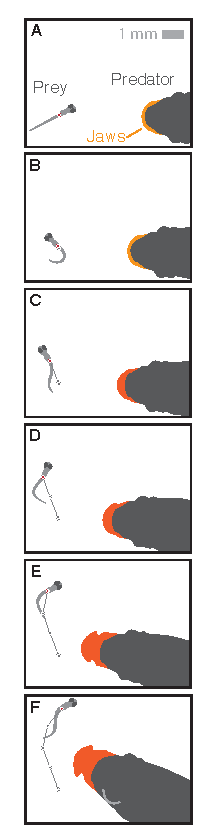
\includegraphics[width=1\textwidth]{Fig_01.pdf}
\centering	
\caption{\textbf{The Homicidal Chauffeur model, applied to prey strategy.} \textbf{(A)} Simulations predict the direction of a prey's fast start relative to initial position and velocity of a predator. \textbf{(B)} Numerical simulations were run at varying escape angle and predator approach speed to examine variation in the minimum distance. At $K>1$, the optimal angle }
\label{weihs_topo}
\end{centering}
\end{figure}

\pagebreak






\end{document}